%!TEX root = ../master.tex
\section{The neighbor attacking the consumer}

If the consumer has some noisy habits, the neighbor may become irritated on his practices.
Gaining access to the smart meter will make it possible to either shut off devices completely or control the devices.
That way he can change the schedules to a better point in time (according to him) or turn down the volume of some device.

The attack tree describing the attack can be found on \cref{fig:attack_trees:neighbor}.
The subtree describing how to get access to the smart meter is identical to that of the burglar, which was described in more detail in \cref{compromise:SM}.

\begin{figure}[h]
  \centering
	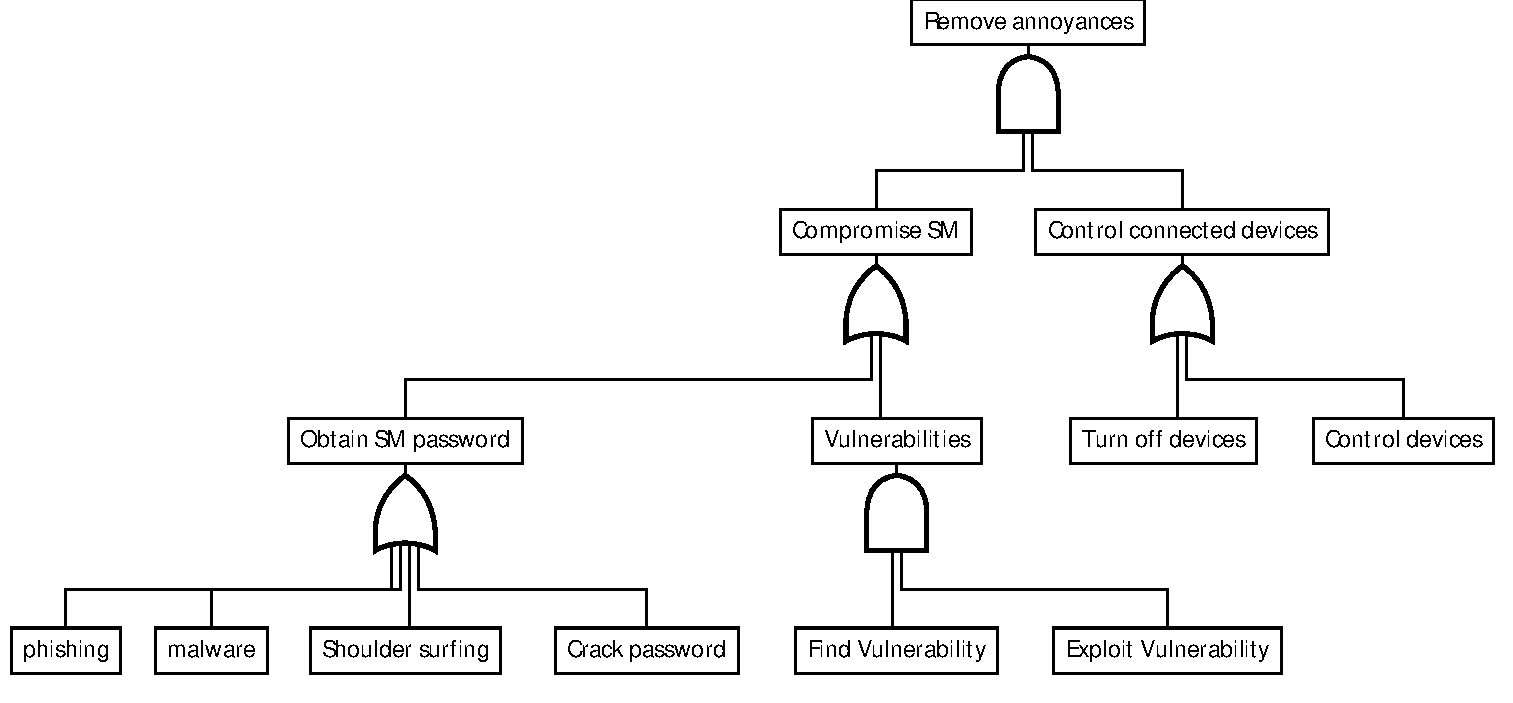
\includegraphics[width=\textwidth]{figures/graphviz/neighbor_vs_consumer.pdf}
	\caption{The neighbor attacking the consumer by turning off or controlling his devices.}
	\label{fig:attack_trees:neighbor}
\end{figure}